\documentclass[]{article}
\usepackage{lmodern}
\usepackage{amssymb,amsmath}
\usepackage{ifxetex,ifluatex}
\usepackage{fixltx2e} % provides \textsubscript
\ifnum 0\ifxetex 1\fi\ifluatex 1\fi=0 % if pdftex
  \usepackage[T1]{fontenc}
  \usepackage[utf8]{inputenc}
\else % if luatex or xelatex
  \ifxetex
    \usepackage{mathspec}
  \else
    \usepackage{fontspec}
  \fi
  \defaultfontfeatures{Ligatures=TeX,Scale=MatchLowercase}
\fi
% use upquote if available, for straight quotes in verbatim environments
\IfFileExists{upquote.sty}{\usepackage{upquote}}{}
% use microtype if available
\IfFileExists{microtype.sty}{%
\usepackage{microtype}
\UseMicrotypeSet[protrusion]{basicmath} % disable protrusion for tt fonts
}{}
\usepackage[margin=1in]{geometry}
\usepackage{hyperref}
\hypersetup{unicode=true,
            pdftitle={Project 3},
            pdfborder={0 0 0},
            breaklinks=true}
\urlstyle{same}  % don't use monospace font for urls
\usepackage{longtable,booktabs}
\usepackage{graphicx,grffile}
\makeatletter
\def\maxwidth{\ifdim\Gin@nat@width>\linewidth\linewidth\else\Gin@nat@width\fi}
\def\maxheight{\ifdim\Gin@nat@height>\textheight\textheight\else\Gin@nat@height\fi}
\makeatother
% Scale images if necessary, so that they will not overflow the page
% margins by default, and it is still possible to overwrite the defaults
% using explicit options in \includegraphics[width, height, ...]{}
\setkeys{Gin}{width=\maxwidth,height=\maxheight,keepaspectratio}
\IfFileExists{parskip.sty}{%
\usepackage{parskip}
}{% else
\setlength{\parindent}{0pt}
\setlength{\parskip}{6pt plus 2pt minus 1pt}
}
\setlength{\emergencystretch}{3em}  % prevent overfull lines
\providecommand{\tightlist}{%
  \setlength{\itemsep}{0pt}\setlength{\parskip}{0pt}}
\setcounter{secnumdepth}{0}
% Redefines (sub)paragraphs to behave more like sections
\ifx\paragraph\undefined\else
\let\oldparagraph\paragraph
\renewcommand{\paragraph}[1]{\oldparagraph{#1}\mbox{}}
\fi
\ifx\subparagraph\undefined\else
\let\oldsubparagraph\subparagraph
\renewcommand{\subparagraph}[1]{\oldsubparagraph{#1}\mbox{}}
\fi

%%% Use protect on footnotes to avoid problems with footnotes in titles
\let\rmarkdownfootnote\footnote%
\def\footnote{\protect\rmarkdownfootnote}

%%% Change title format to be more compact
\usepackage{titling}

% Create subtitle command for use in maketitle
\newcommand{\subtitle}[1]{
  \posttitle{
    \begin{center}\large#1\end{center}
    }
}

\setlength{\droptitle}{-2em}
  \title{Project 3}
  \pretitle{\vspace{\droptitle}\centering\huge}
  \posttitle{\par}
  \author{}
  \preauthor{}\postauthor{}
  \date{}
  \predate{}\postdate{}


\begin{document}
\maketitle

\section{Introduction}\label{introduction}

This is Project 3 for STAT 557 2018 Spring by Meridith Bartley and Fei
Jiang. The aim of this project is to implement a tree structured
classifier using the splitting method in CART and a chosen split
stopping criterion and then apply this classifier to a data set.

\section{Description of Data}\label{description-of-data}

This car evaluation dataset is developed by Marko Bohanec and Blaz Zupan
(1997). The response variable is the condition of a car which has two
classes: unacceptable and acceptable. There are six predictors to
develop the model: buying price, price of the maintenance, number of
doors, capacity in terms of persons to carry, the size of luggage boot,
and estimated safety of the car.

Boxplots for each numeric attribute (doors, persons) used as explanitory
variables in the subsequent classification models are included below.
This EDA allows for early indication of which variables may possibly be
ommitted during dimention reduction. That is, what properties do not
differ significantly between safety classifications.

\subsection{Exploritory Data Analysis}\label{exploritory-data-analysis}

An initial examination of the data reveals no missing data (as no NA
values were present). Also, the already present classification indicates
that 518 cars (30\% of the given data) were in an acceptable condition,
while the remaining 1210 cars (70\% of the given data) are seen to be
unacceptable.

The colored bar charts below show the requency of cars within each
category of four difference qualitative variables, split by condition.
Some initial revealed relationships include car in acceptable conditions
seeming having lower costs of both buying and maintainance. In addition,
we note that cars with low safety ratings are exclusively in
unacceptable conditions. These initial observations are in line with
intuative preferences for cars; people want safe, convienent cars for a
low price.

The black and white box plots show the spready of car data for each of 2
quantitative variabless, again split by condition. We note that
acceptable cars are only observed to have 4 or 5 doors, in addition cars
in acceptable condition are more likely to have an increased number of
doors. This increased door count may correlate with the car size and
thus the overall safety of the car.

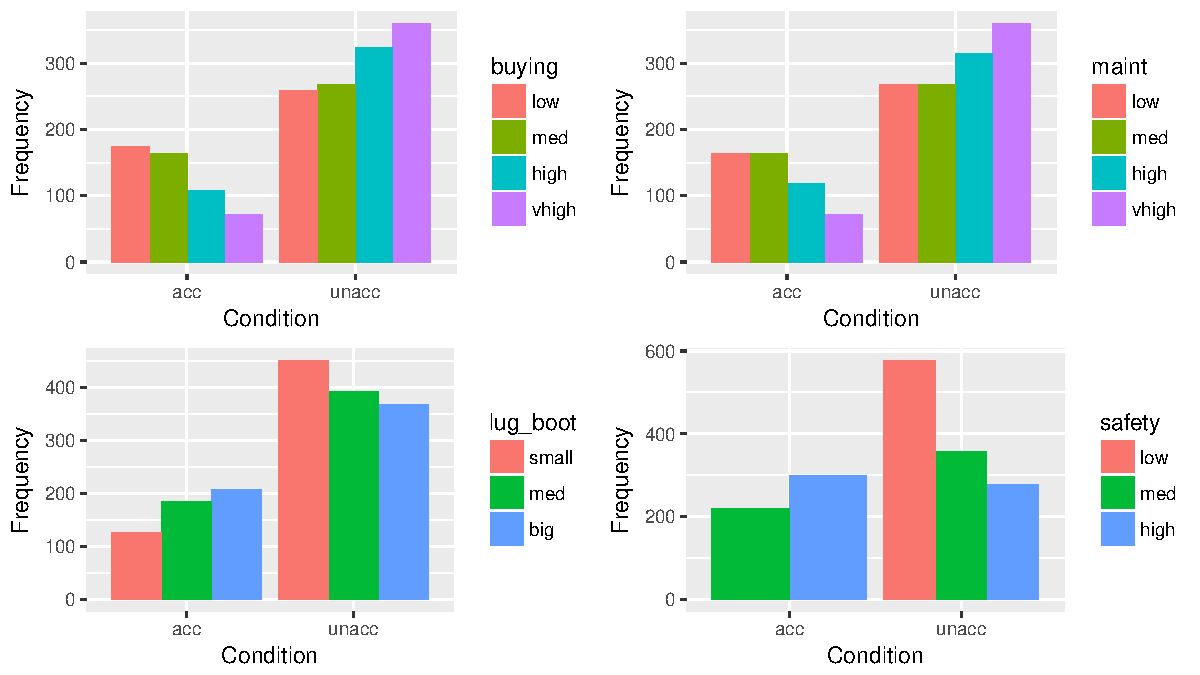
\includegraphics{Project3_files/figure-latex/EDA - Fei-1.pdf}
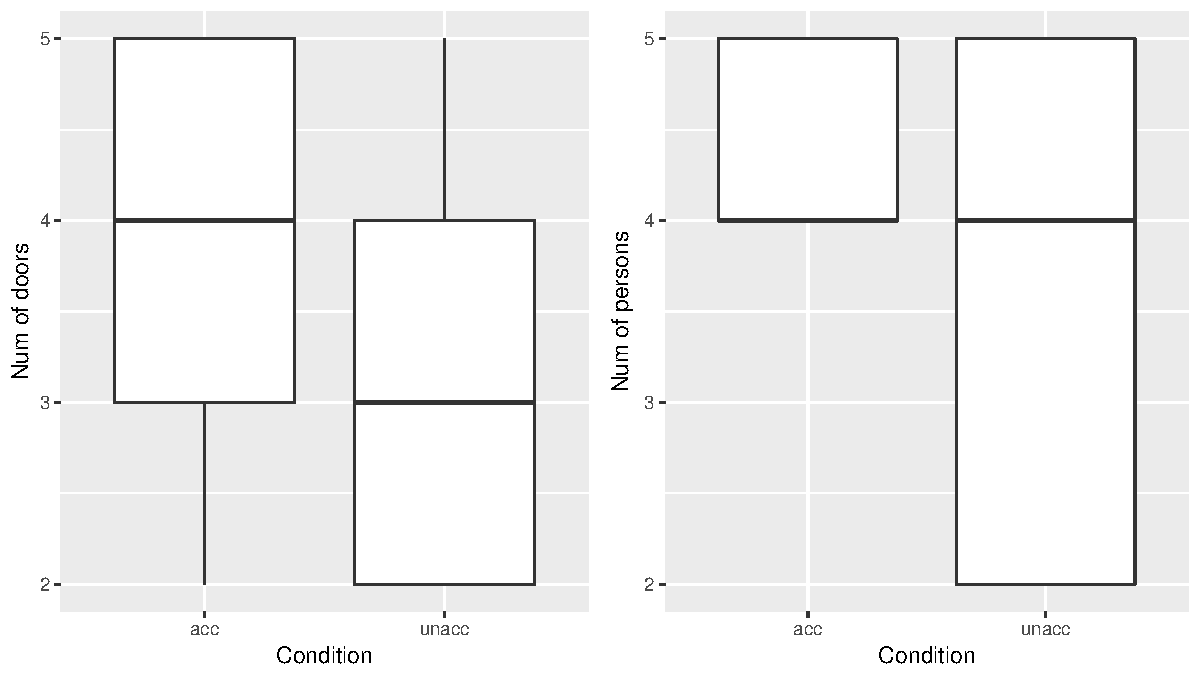
\includegraphics{Project3_files/figure-latex/EDA - Fei-2.pdf}

\section{Analysis}\label{analysis}

In this project, we will use tree classifier to classify the given data
into acceptable and unaccepable conditions. We divided the given data
into test data (20\% of the given data) and training data (80\% of the
given data) after randomizing the overall dataset. Prediction accuracy
will be determined by assessing the total misclassification rate on the
training and test data.

A tree based method can be used to predict the expected value of either
a qualitative response (classification tree) or a quantitative response
(regression trees). However, as our given data set has a qualitative
response, we shall focus on classification trees. We predict that each
observation belongs to the most commonly occurring class of training
observations in the region to which it belongs. In interpreting the
results of a classification tree, we are often interested not only in
the class prediction corresponding to a particular terminal node region,
but also in the class proportions among the training observations that
fall into that region. Since we plan to assign an observation in a given
region to the most commonly occurring class of training observations in
that region, the classification error rate is simply the fraction of the
training observations in that region that do not belong to the most
common class.

\subsection{Pseudo-code of the tree structured
classifier}\label{pseudo-code-of-the-tree-structured-classifier}

Our classifier tree is grown as follows:

\begin{enumerate}
\def\labelenumi{\arabic{enumi}.}
\item
  A single variable is found which best splits the data into two groups
  (`best' will be defined later).
\item
  The data is separated, and then this process is applied separately to
  each sub-group.
\item
  Continue recursively until the subgroups either reach a minimum size
  or until no improvement can be made.
\item
  Pick the tree size that minimizes misclassification rate
  (i.e.~prediction error).
\item
  Prune the tree using the best complexity parameter. Here, the
  complexity parameter means that if any split does not increase the
  overall R-square of the model by at least \#complexity parameter\#
  (where R-square is the usual linear-models definition) then that split
  is decreed to be, a priori, not worth pursuing. This parameter allows
  us to avoid over-fitting.
\end{enumerate}

\subsection{Apply tree classifier to the example
dataset}\label{apply-tree-classifier-to-the-example-dataset}

The unpruned (top plot) and pruned (bottom plot) tree developed based on
training dataset are shown below. They both show that the number of
people a car can carry and the safety level are very critical to
determine whether a car is acceptable or not. But the pruned tree is
simpler and easier to interpret and apply because some unimportant
branches have been pruned.

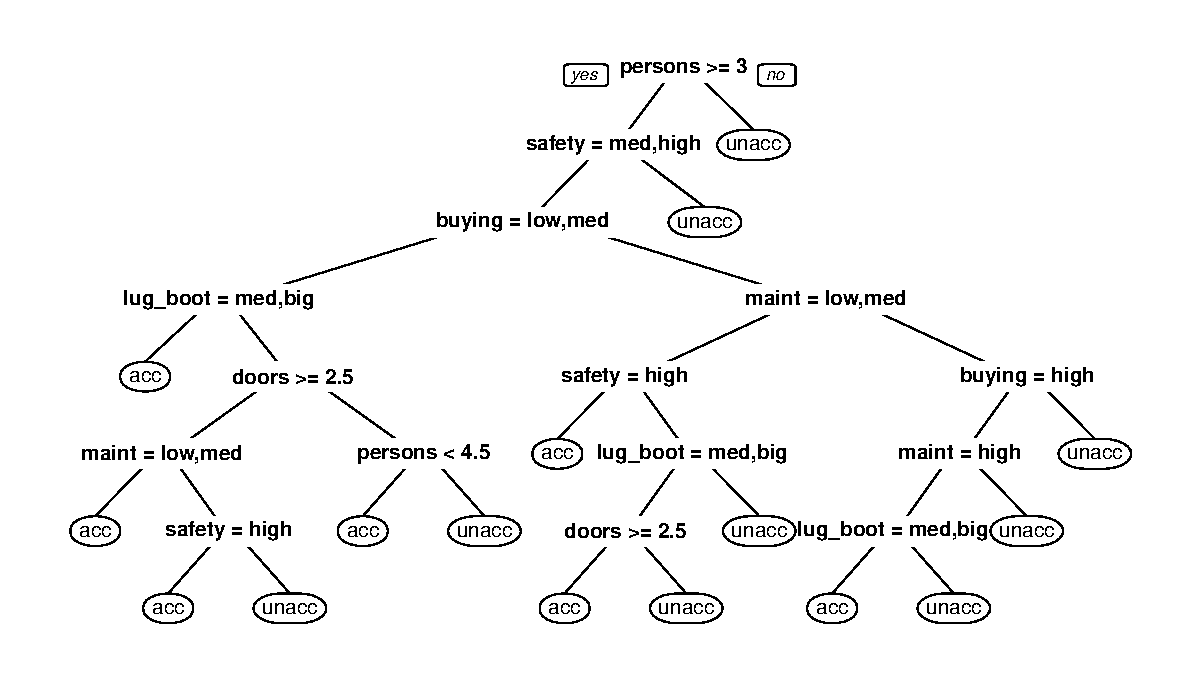
\includegraphics{Project3_files/figure-latex/Classifier - Fei-1.pdf}
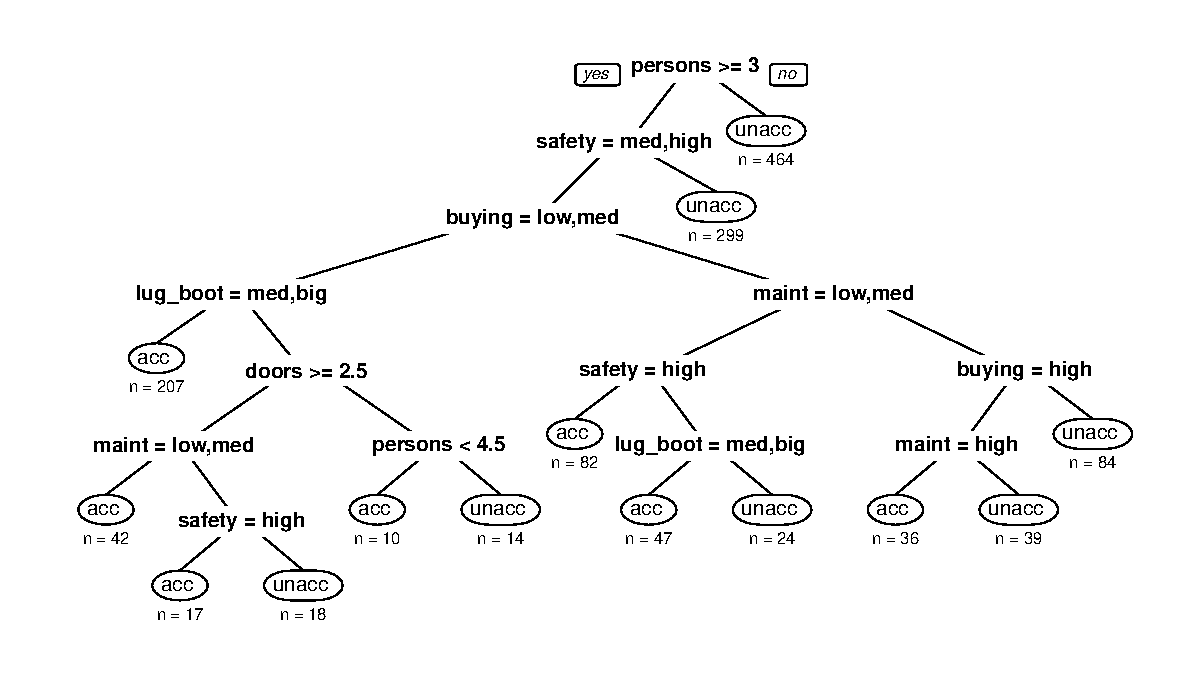
\includegraphics{Project3_files/figure-latex/Classifier - Fei-2.pdf}

\section{Conclusions}\label{conclusions}

The above trees represent the resulting unpruned (top) and pruned
(bottom) trees for classifying cars into either acceptable or
unacceptable conditions. Several of the initial splits (number of
persons and safety rating) reflect the stark differences between
conditions that were revealed in the EDA above. With just these two
splits the majority (763) of the unacceptable condition cars have been
identified. Our unpruned tree has 15 splits while our pruned tree has
just 13 splits.

The confusion matrices below show the accuracy of the pruned tree's
predicitons for the training (top) and testing (bottom) datasets. We
observed a prediciton error rate of 2.60\% in the training data and of
2.89\% in the testing data. We consider minimizing misclassification
rates to be vital with these car condition classification data as the
consequences of purchasing/driving in an unacceptable car includes a
risk to one's personal safety.

\begin{longtable}[]{@{}lrr@{}}
\toprule
& Pred:acc & Pred:unacc\tabularnewline
\midrule
\endhead
Actual:acc & 410 & 5\tabularnewline
Actual:unacc & 31 & 937\tabularnewline
\bottomrule
\end{longtable}

\begin{longtable}[]{@{}lrr@{}}
\toprule
& Pred:acc & Pred:unacc\tabularnewline
\midrule
\endhead
Actual:acc & 102 & 1\tabularnewline
Actual:unacc & 9 & 233\tabularnewline
\bottomrule
\end{longtable}

\section{Contributions}\label{contributions}

The different tasks required to complete this project were equally
divided between Meridith and Fei. Both members of this group contributed
to this report and the presentation.


\end{document}
